\chapter{Problemi inversi}

\section{Problemi diretti}
Nel mondo reale i vari fenomeni sono descritti dalla fisica attraverso un problema diretto come 
\[
    \text{causa} \to \text{modello} \to \text{effetto}     
\]
Per esempio, se voglio calcolare l'accelerazione di un'auto, ne individuo i vari passaggi
\begin{itemize}
    \item La causa: ovvero la forza generata dal motore
    \item Modello: la leggi di newton che forniscono le formule e le leggi apposite (supponendo un sistema inerziale)
    \item Effetto: calcolo dell'accelerazione
\end{itemize}

Quindi acquisisco in input l'origine dell'effetto (ovvero la forza) attraverso un modello (leggi di newton) elaboro questo dato ed infine ne calcolo l'effetto finale (l'accelerazione). In si può scrivere "matematichese": $x \to A \to y$, che traslato in algebra lineare si ha così:
\[
    Ax \to y    
\]
Si giunge così alla definizione di \textbf{problema diretto}
\dfn{}{
Si definisce \textbf{problema diretto} il processo mediante il quale si determina l'effetto dato un sistema e le cause iniziali
}
In altre parole: input -> output

\section{Problemi inversi}

D'altra parte esistono dei casi in cui si riesce solo ad osservare l'effetto di un fenomeno ed occorre, partendo da questo, risalire alla causa, da questo concetto abbiamo la definizione di \textbf{problema inverso}

\dfn{}{
    Un \textbf{problema inverso} è un tipo di problema matematico3 in cui, dato l'effetto o l'output osservato, si cerca di determinare le cause o i parametri del sistema che lo hanno generato
}

Che in termini matematici significa determinare una $x$ conoscendo $A$ e $y$, ovvero output -> input.

Tuttavia \red{nel mondo reale i dati $y$ sono sempre affetti da errore (detto anche \textbf{rumore})} rappresentato dal vettore $\delta$ che non sono solo errori di rappresentazione ma anche legati a problemi di tipo fisico, forti di questa consapevolezza il problema diventa quindi:

\[
    Ax = y+\delta = y^\delta    
\]

\subsection{Problemi inversi lineari con matrici mal condizionate}

Vi sono delle classi di problemi la cui matrice $A$ relativa al modello matematico del problema è mal condizionata, tali problemi si dicono \textbf{mal posti}. In questo caso il problema viene risolto come un problema di minimi quadrati (che permette di avere anche una matrice rettangolare):
\[
    min_x\|Ax - y^\delta\|_2^2
\]

la cui soluzione è
\[
    x^*=\sum_{i=1}^{n} \frac{u^T_iy^\delta}{\sigma_i}v_i    
\]

\subsection{Perturbazione dell'errore}

A causa di un mal condizionamento di $A$ si ha che, in presenza di un errore  $\delta$, si ha che questo errore venga eccessivamente amplificato nella soluzione dei minimi quadrati
\esempio{
    Si consideri una soluzione "vera" (ground truth) denotata con $x_{GT}$ a cui si applica una matrice $A$ che rappresenta il sistema di acquisizione dati per ottenere il vettore $y:Ax = y$ 

    Al vettore $y$ si aggiunge un vettore $\delta$ che rappresenta il rumore e che e’ preso come vettore random da una distribuzione normale con media nulla: $y^\delta = y + \delta$

    Ecco il grafico di questo scempio:
    \begin{center}
        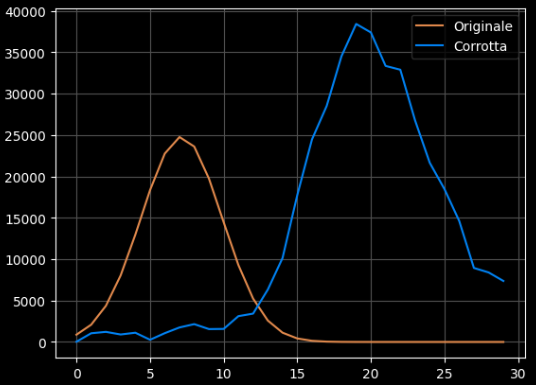
\includegraphics[width=10cm]{img/errore_amplificato.png}    
    \end{center}
    
}

Questo accade perché quando una matrice $A$ è mal condizionata \red{i suoi valori singolari $\sigma_i$ sono molto piccoli, pertanto il numeratore della sommatoria è molto grande}, per capire meglio si osservino i calcoli:
\[
    \min_x\|Ax - y^\delta\|_2^2 = min_x\|Ax - (y+\delta)\|_2^2     
\]
La cui soluzione è:
\[
    x^*=\sum_{i=1}^{n} \frac{u^T_iy^\delta}{\sigma_i}v_i = \sum_{i=1}^{n} \frac{u^T_i(y+\delta)}{\sigma_i}v_i = \sum_{i=1}^{n} \frac{u^T_iy}{\sigma_i}v_i + \sum_{i=1}^{n} \frac{u^T_i\delta}{\sigma_i}v_i
\]

È proprio la seconda sommatoria il problema! È facile verificare che più i $\sigma_i$ sono piccoli più $u^T_i\delta$ è matematicamente "amplificato"
\subsubsection{Condizioni di Picard}
La \textbf{condizione discreta di Picard} è un criterio utilizzato per diagnosticare la "malcondizionatura" nei problemi inversi lineari e per capire la stabilità della soluzione. La condizione discreta di Picard si basa sull'analisi dei \red{valori singolari $\sigma_i$ e i cosidetti coefficienti di Fourier $u_i^Ty^\delta$} 

\dfn{}{
    La \textbf{condizione discreta di Picard} afferma che che, affinché il problema sia ben posto, i coefficienti di Fourier  $u_i^Ty^\delta$devono decrescere almeno altrettanto velocemente dei valori singolari $\sigma_i$
}

\esempio{
    Si consideri questo esempio:
    
    \begin{center}
        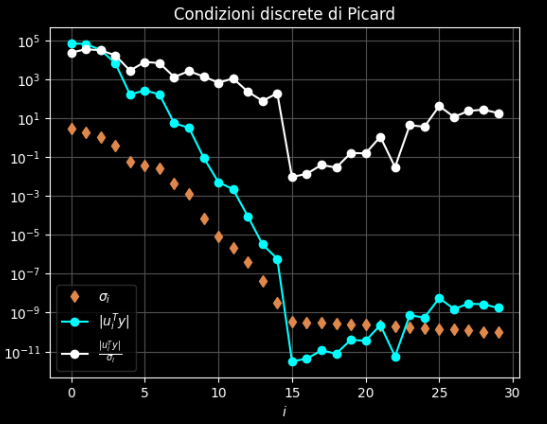
\includegraphics[width=10cm]{img/picard.png}
    \end{center}

    In questo caso la condizione di Picard è rispettata fino all’ indice $i=15$

    Si consideri quest'altro esempio:
    \begin{center}
        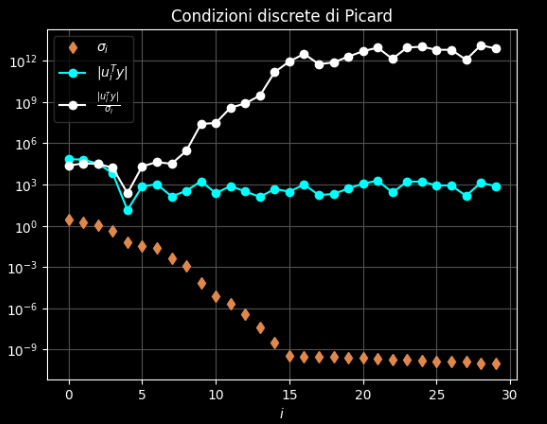
\includegraphics[width=10cm]{img/picard_2.png}
    \end{center} 
    In questo caso la condizione di Picard è rispettata fino all’ indice $i=5$
  
}

\subsection{Metodi di regolarizzazione}
Per affrontare la malcondizionatura e ottenere una soluzione più stabile e accettabile, è \red{necessario modificare il problema attraverso tecniche dette metodi di regolarizzazione}. Esistono diverse tecniche di regolarizzazione, verrano riportate qui sotto

\subsubsection{Decomposizione in Valori Singolari Troncata}

Nel metodo di regolarizazione denominato TSVD (Truncated Singular Value Decomnposition) la soluzione del problema di minimi quadrati: 
\[
    min_x \|Ax - y^\sigma\|_2^2    
\]
viene calcolata come:
\[
    x_{TSVD} = \sum_{i=1}^{K} \frac{u_i^T y^\delta}{\sigma_i} v_i  
\]
Con $K < n$.
Posso anche scrivere la soluzione come:
\[
    x_{TSVD} = \sum_{i=1}^{n} f_i\frac{u_i^T y^\delta}{\sigma_i} v_i  
\]
dove i coefficienti $f_i$ sono detti \textbf{fattori di filtro}, dove in questo caso sono dati da:
\[
    f_i = \begin{cases}
        1 & i\leq K\\
        0 &  i>K
    \end{cases}    
\]

E dove un buon valore $K$ è quello dopo il quale non sono più soddisfatte le condizioni di Picard 

\subsubsection{Regolarizazione di Tikhanov}
La \textbf{regolarizzazione di Tikhonov}, invece, utilizza fattori di filtro che siano numeri in
$[0, 1]$ e che quindi “pesino” le componenti della somma in modo piu’ graduale. In
particolare,\red{ devono essere pesate di più le componenti di indice piccolo, associate ai
valori singolari più grandi, e meno quelle di indice grande, associate ai valori singolari
piu’ piccoli}

Il problema diventa quindi:
\[
    x_{tikh} =  min_x \|Ax - y^\sigma\|_2^2   + \lambda\|Lx\|_2^2
\]
Dove:
\begin{itemize}
    \item $\lambda>0$ è il parametro di regolarizzazione che pesa la parte di congruenza con i dati e la parte di regolarità della soluzione
    \item $L$ è la matrice Identità
\end{itemize}

Si può anche scrivere in questo modo:
\[
    x_{tikh} =  min_x \|Mx - Y\|_2^2 
\]
Dove:\begin{itemize}
    \item $M$ è la matrice di dimensione $2m \times n$ che ha come blocchi in colonna rispettivamente la matrice $A$ e la matrice $\lambda I$
    \item $Y$ è il vettore di dimensione $2m$ che ha
    come vettori colonna rispettivamente $y^\delta$ e il vettore nullo
\end{itemize}

Si può inoltre dimostrare che  la soluzione di Tikhonov posso anche scriverla tramite i fattori di filtro come:
\[
    x_{tikh} = \sum_{i=1}^{n}     f_i \frac{u^T_i y^\delta}{\sigma_i}v_i
\]
dove:
\[
    f_i = \frac{
        \sigma^2_i
    }{
        \sigma^2_i + \lambda  
    }
\]
\subsubsection{Principio di maassima discrepanza}

Si giunge, tuttavia, ad un problema: la scelta del parametro di regolarizzazione nel metodo di Tikhonov. Infatti questa scelta è sicuramente la parte piu’ delicata della
regolarizzazione, un parametro troppo piccolo non
toglie il rumore dalla soluzione, mentre un parametro troppo grande produce una
soluzione troppo regolare, in cui non e’ piu’ presente il rumore ma per esempio le
oscillazioni o i picchi che ci sono nella soluzione esatta vengono troppo ridotti.

\red{Teoricamente il valore ottimale del parametro $\lambda_{opt}$ è quello che minimizza:}
\[
    \lambda_{opt} = \min_\lambda\|x_\lambda - x_{GT}\|_2^2
\]
dove $x_\lambda$ è la soluzione calcolata in corrispondenza di un certo $\lambda$.

Non esiste un metodo sempre efficiente per scegliere il parametro di regolarizzazione.
Sicuramente in pratica spesso si usa una tecnica euristica che consiste nel provare
alcuni parametri e scegliere quello che produce la soluzione che ci sembra migliore (trial and test). La tecnica sicuramente più utilizzata in pratica è il principio di massima discrepanza.

\dfn{}{
    Il \textbf{Principio di Massima Discrepanza} afferma che il parametro di regolarizzazione $\lambda$ dovrebbe essere scelto in modo tale che la norma del residuo (cioè la differenza tra i dati osservati e quelli ricostruiti) sia proporzionale alla stima della norma del rumore nei dati

    Formalmente:
    \[
        \|Ax_\lambda - y^\delta \| = v_{DP} |\delta|_2^2
    \]
    Dove: 
    \begin{itemize}
        \item $x_\lambda$ è la soluzione regolarizzata con parametro $\lambda$
        \item $v$ è un fattore di proporzionalità (spesso scelto vicino a 1)
        \item $\|\delta\|$ è la norma dell'errore (spesso è impossibile conoscerla ma si può fare una stima)
    \end{itemize}
}

Quindi \red{il residuo deve essere uguale alla norma del rumore, quindi provo tanti $\lambda$, quello più vicino a questa soluzione è quello migliore}
